\chapter{Implementation}

To implement our task the programming language C++ combined with openCV was used. Further external libraries were not necessary.

\section{Details}

The algorithm procedure can be seen in the \texttt{main.cpp} file where all used classes are generated and sequentially executed.\\\\

Generally the following variables (vectors of cv::Mat objects) are declared at the beginning:


\begin{itemize}
\item image\_set
\item transformed\_set
\item transformed\_gray\_set
\item foreground\_set
\end{itemize}

where the image\_set vector of matrices is filled with the raw input image data. The transformed\_set and the according gray valued vector are then filled with the preprocessed images which means that all additional images are transformed and matched to the first image (first image is defined as key image). The foreground\_set variable represents the foreground mask which is computed in the end of our algorithm.\\\\

To provide useful image data for further computation the image sequence has to be transformed (matched) with the key image. For this the class \texttt{Preprocessor} was introduced which smooths the images and calculates salient points to match them between every "next" image and the first image. This is done by using the FAST detector and the SURF descriptor to get sufficiently discriminative features. These are matched with the FLANN based matcher provided by openCV. Further, only good matches (thresholding) are used to estimate the homography for warping the images (perspective transformation).\\\\

After this preprocessing the transformed\_set (shich includes the transformed color images) and the transformed\_gray\_set (gray valued image set) can be used for calssification between background and foreground. This is handled by the virtual class classifier from which certain classes can be derived (HSVVarianceForegroundClassifier, ColorVarianceClassifier, TestForegroundClassifier). This was useful for applying different approaches and experimenting witch parameters to find the best method. The choice was made for the ColorVarianceClassifier method which uses RGB data. Basically the classifier class detects foreground pixels and sets the foreground\_set variable (foreground mask).\\\\

Up to here we already detected the likely foreground which has to be ignored. Now the question arises how to blend/fill the foreground gaps of the key image. This is done by the class inPainter. The method \texttt{InPainter::inpaint(...)} is using the euclidean distance transformation for blending the borders (alpha blending method).\\
For the rare case that a pixel is detected as foreground in every image we used the $L_1$ minimizer corresponding to the median of all pixel values considering all images.


\chapter{Evaluation/Results}

To get an imagination of the influence of the parameter $\alpha$ which is used by our cost function $f(\Omega)$ can be seen in the following picture sequence.

\begin{figure}[h!t]
\centering
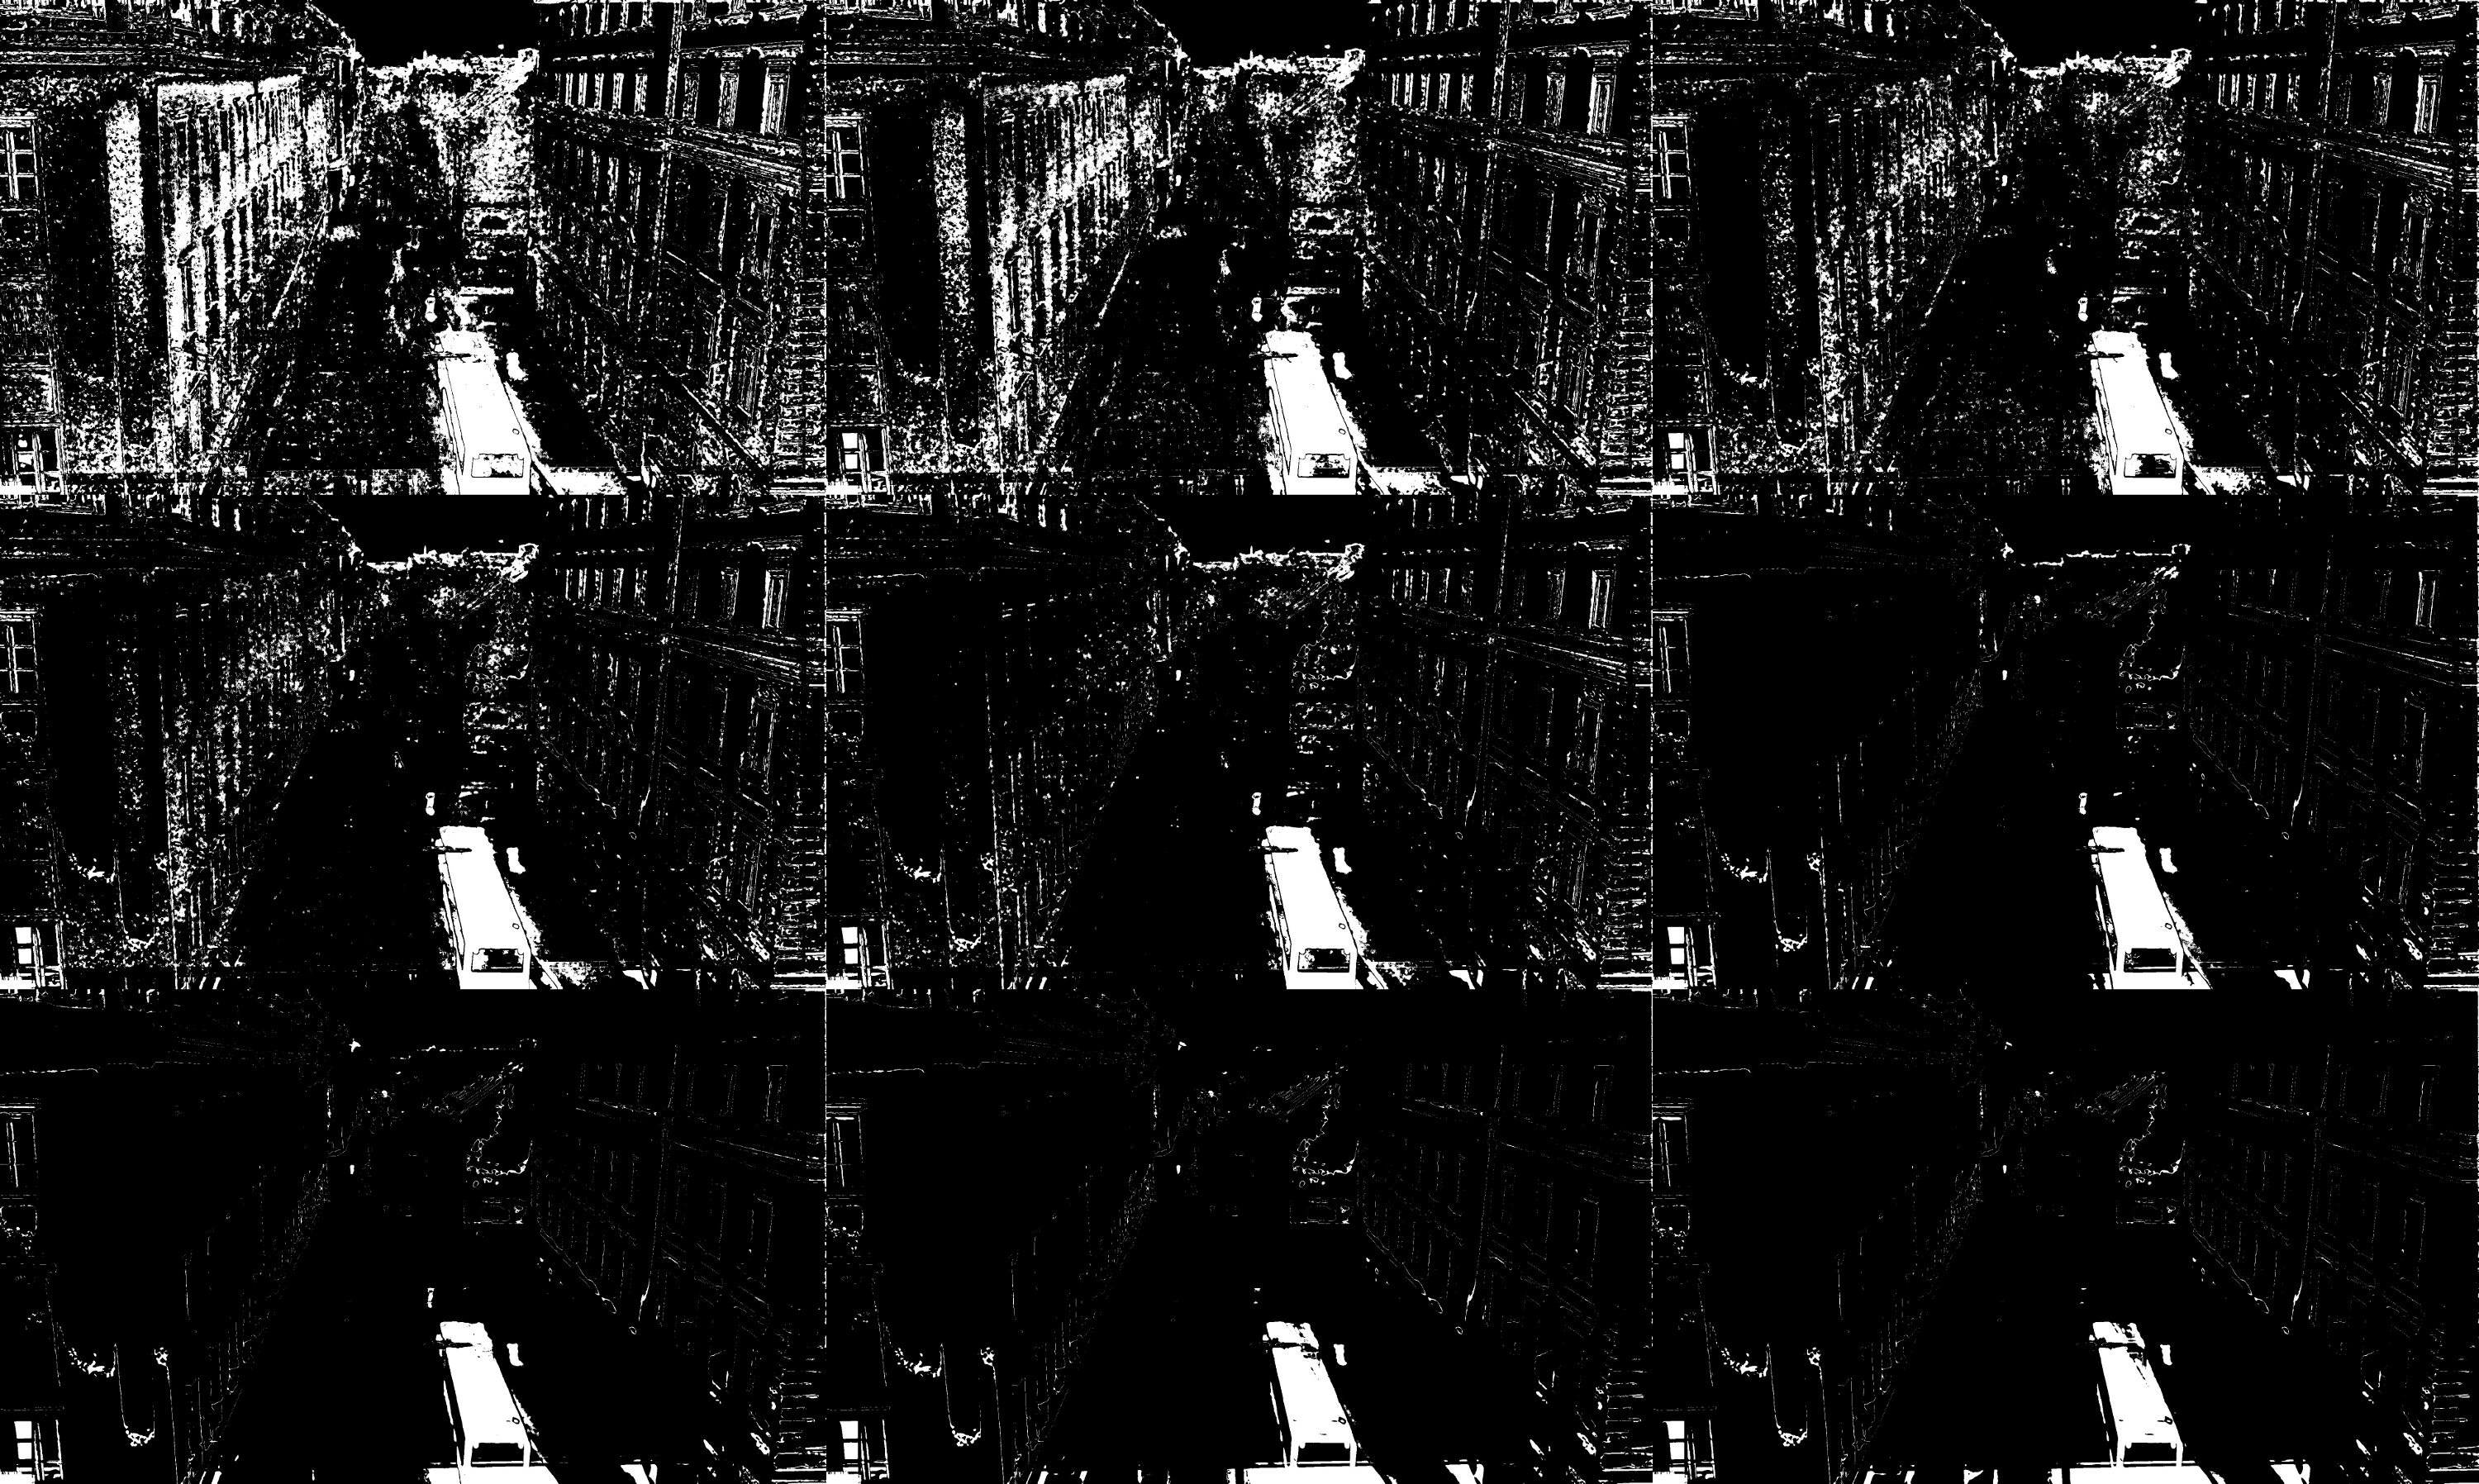
\includegraphics[scale = 0.14]{pics/alpha.jpg}
\caption{The influence of parameter $\alpha$ by increasing it}
\label{1}
\end{figure}


The results in the following figures show how nice the algorithm works although we're using only low-level pixel-wise operation by applying our algorithm on some main places in the city Graz (Austria).

\begin{figure}[h!t]
\centering
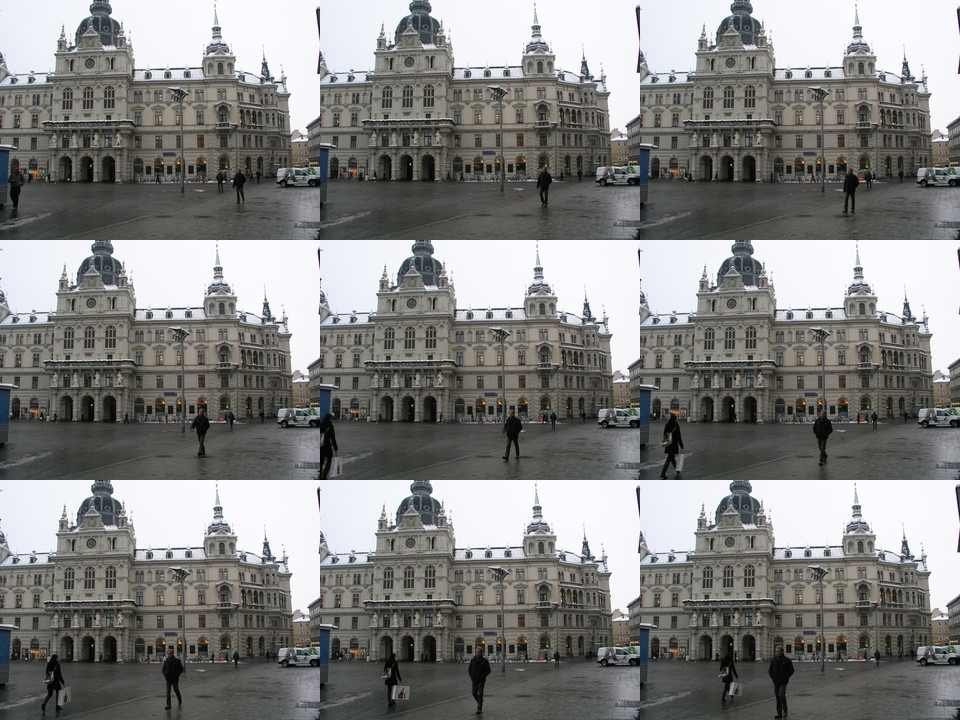
\includegraphics[scale = 0.43]{pics/rathaus.jpg}
\caption{Used input frames for "cleaning" the picture of the city hall in Graz}
\end{figure}

\begin{figure}[h!t]
\centering
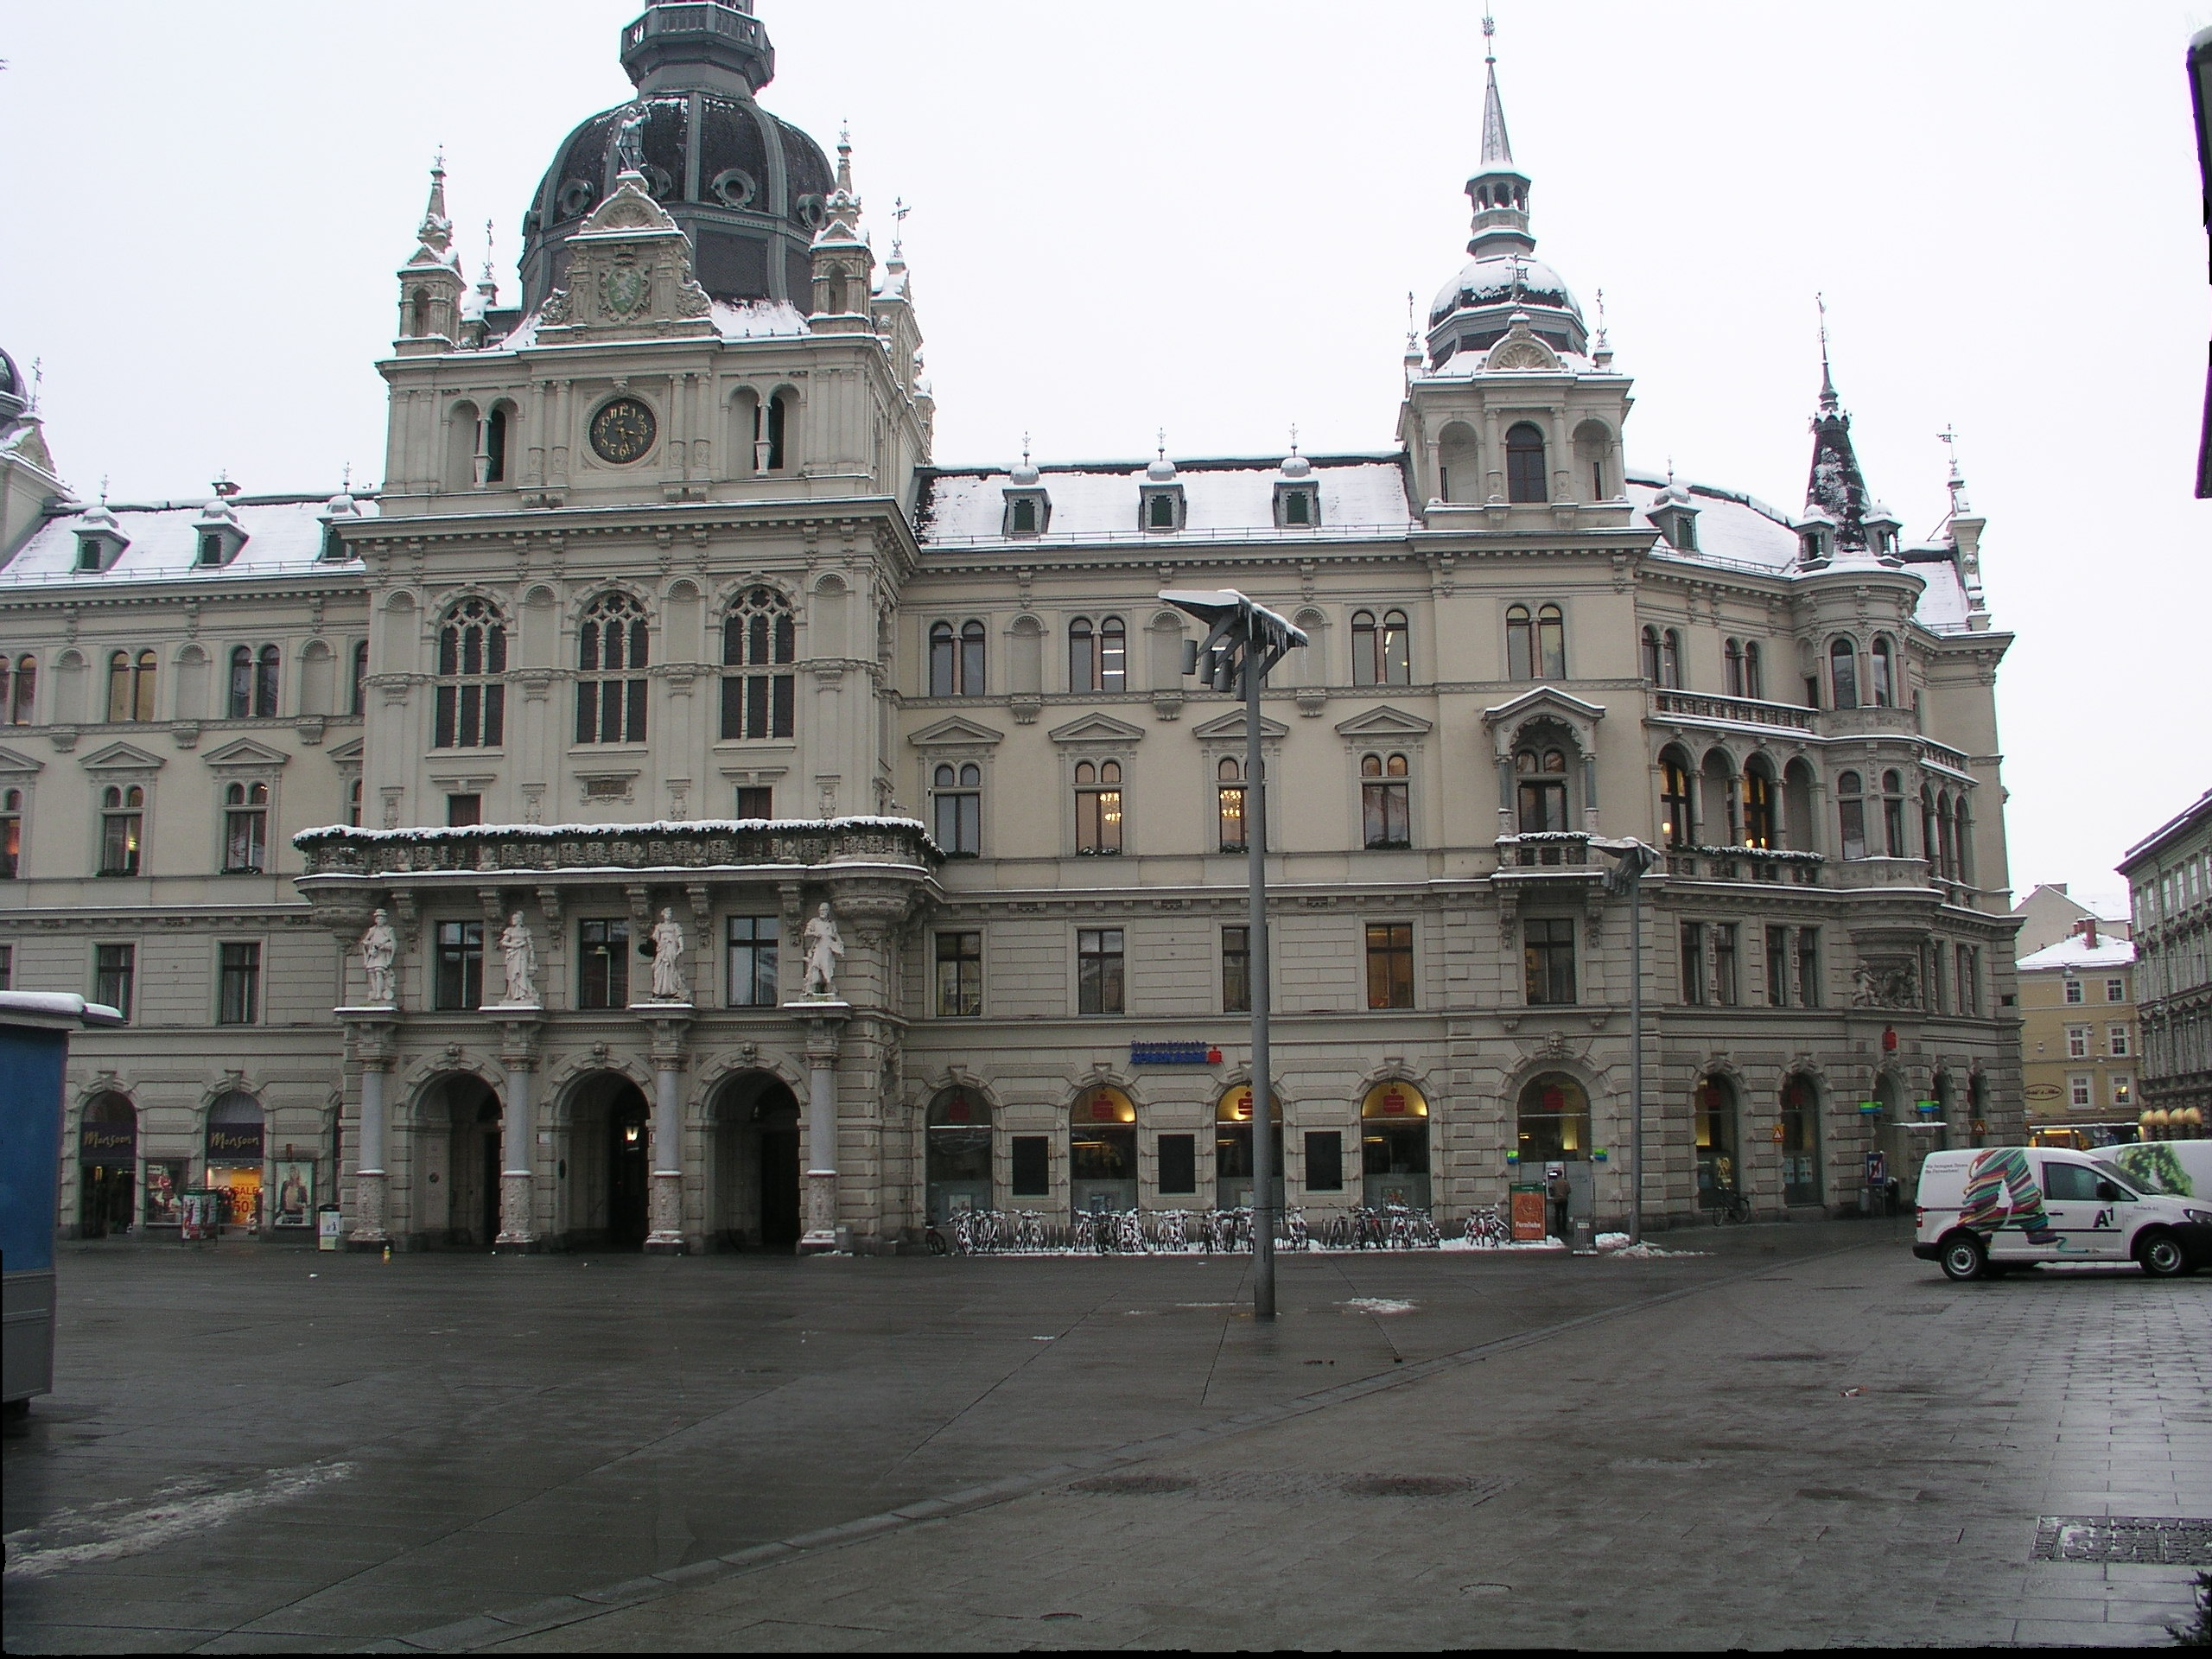
\includegraphics[scale = 0.16]{pics/result.jpg}
\caption{Resulting "cleaned" picture of the city hall of Graz}
\end{figure}

\newpage
As seen satisfiable results can be obtained. Furthermore an extreme test for the \textit{Jakominiplatz} in Graz was done with the following results:

\begin{figure}[h!t]
\centering
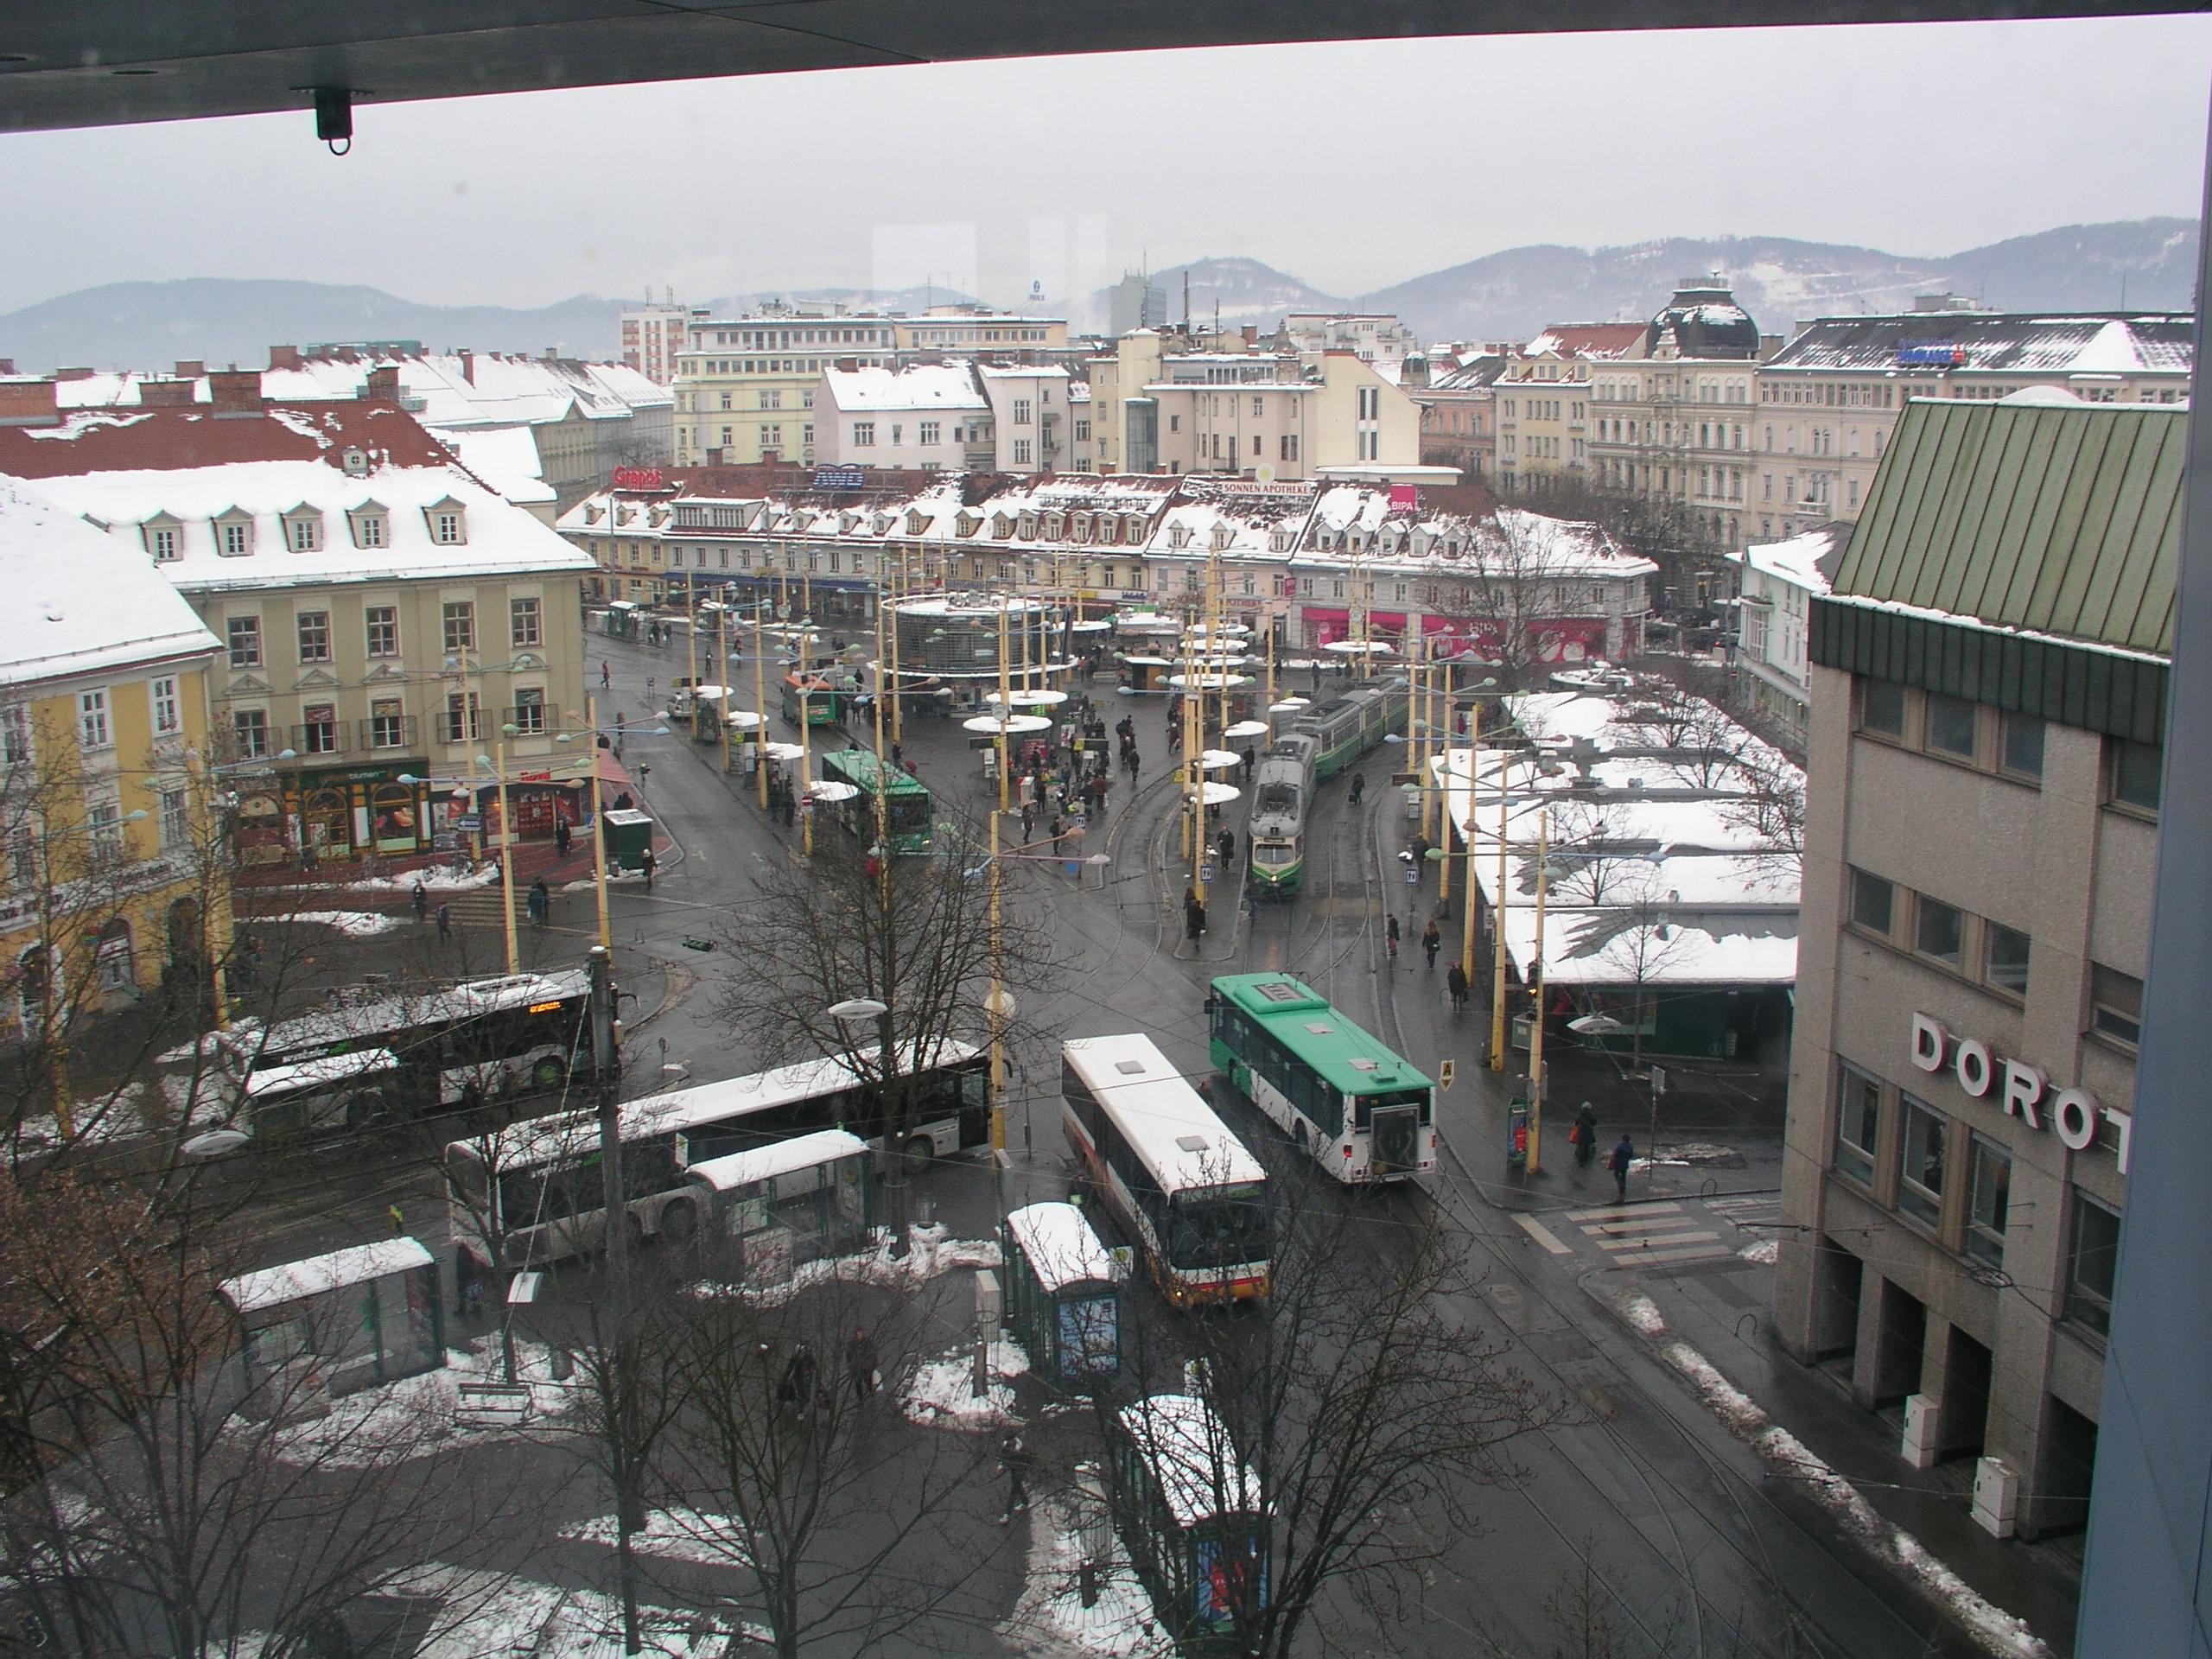
\includegraphics[scale = 0.145]{pics/jako_before.jpg}
\caption{Picture of the \textit{Jakominiplatz} of Graz}
\end{figure}

\begin{figure}[h!t]
\centering
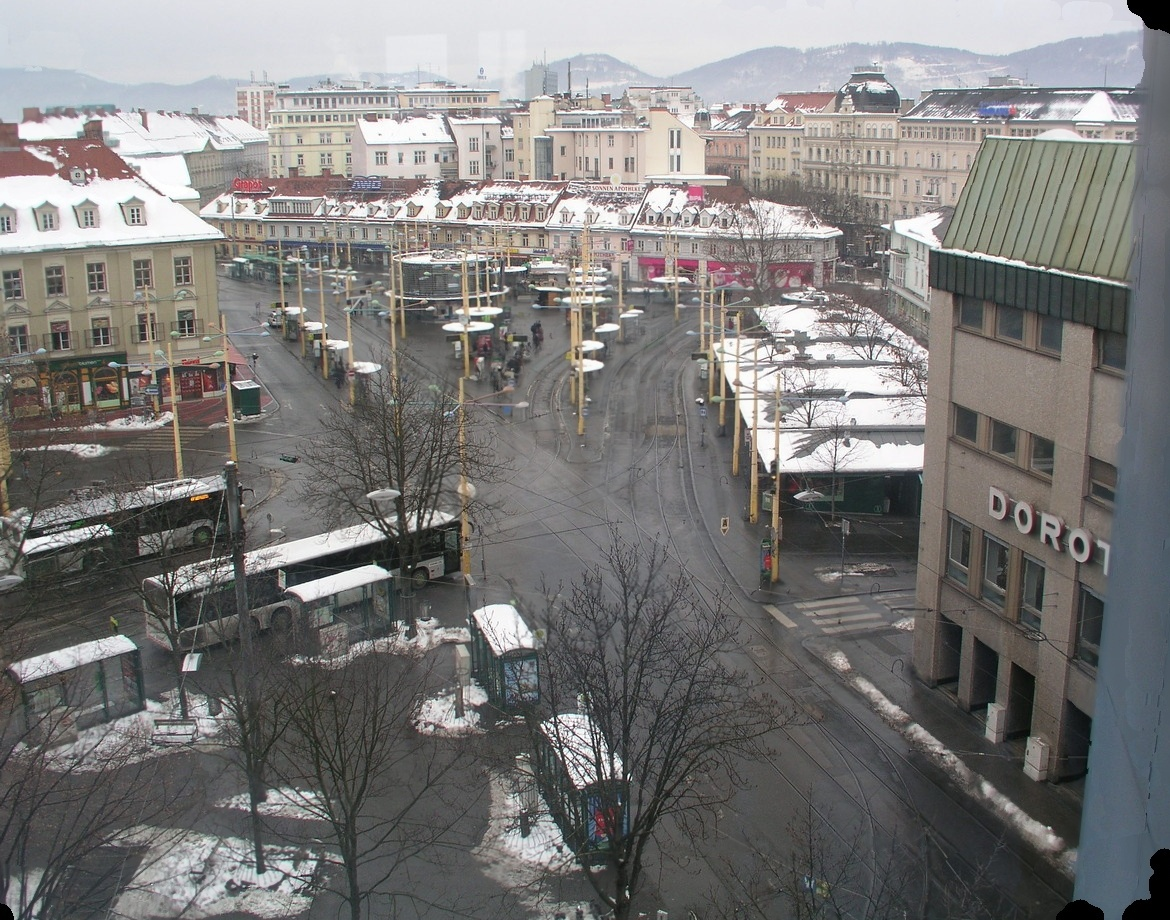
\includegraphics[scale = 0.32]{pics/jako.jpg}
\caption{Resulting "cleaned" picture of the \textit{Jakominiplatz} of Graz}
\end{figure}

Only "waiting" people and standing buses are still in the image..

\chapter{Discussion}

All in all the expected goal was achieved by our implementation as it can be seen in the result images.\\
Nevertheless some problems (which were not expected) did arise. The main problem was/is the in some kind inaccurate estimation of the homography for the image matching. This is a big problem if using pixelwise operations where especially the outer regions of the image are concerned.\\
The next point was to find an appropriate blending mechanism to fill the gaps of the foreground regions. Further we payed attention on the efficiency of our program which lead to more trade-offs between accuracy and speed.\\\\

The limits of our implementation is still dependent on the frequency of foreground such as persons moving through the scene. If many persons cover the background it is still impossible to do a reconstruction which becomes obvious because then also humans are not able to "see" behind obstacles.\\\\

To improve our algorithm we could add additional features for determining/evaluating the overall variance, such as gradient information or edge information. Besides that the neighborhood of each pixel could be included which may lead to more robustness and to better results.


